\subsection{Rancangan Behavioral}

Berdasarkan Use Case yang telah dirumuskan, terdapat 2 skenario utama yang akan dilakukan oleh pengguna, yaitu pencarian Smart Contracts dan pengambilan data address dari Smart Contracts. Selain itu, terdapat juga skenario tambahan yang terjadi di dalam sistem tanpa campur tangan pengguna, yaitu ekstraksi data Smart Contracts dari Blockchain, transformasi data Smart Contracts ke dalam Dgraph Database, Semantic Enrichment pada data Smart Contracts, transformasi data Smart Contracts menjadi vector embeddings, dan penyimpanan vector embeddings ke dalam Vector Database.

\subsubsection{Alur Mencari Smart Contract}

Pengguna akan melakukan pencarian dengan menggunakan API atau GUI. Pengguna akan memasukkan bahasa alami yang mendeskripsikan kebutuhan Smart Contract yang dicari. Data masukan yang diterima akan diteruskan ke API lalu ke komponen Retriever, yang akan melakukan query enrichment dan mengirimkan query ke dalam Vector Database dalam bentuk embedding. Hasil pencarian yang didapatkan akan dikembalikan ke API dan ditampilkan kepada pengguna dalam bentuk tabel yang berisi informasi Smart Contract yang relevan dengan query yang dimasukkan oleh pengguna. Ilustrasi alur pencarian Smart Contract dapat dilihat pada Gambar \ref{image:alur-pencarian-smart-contract}.

\begin{figure}[ht]
    \centering
    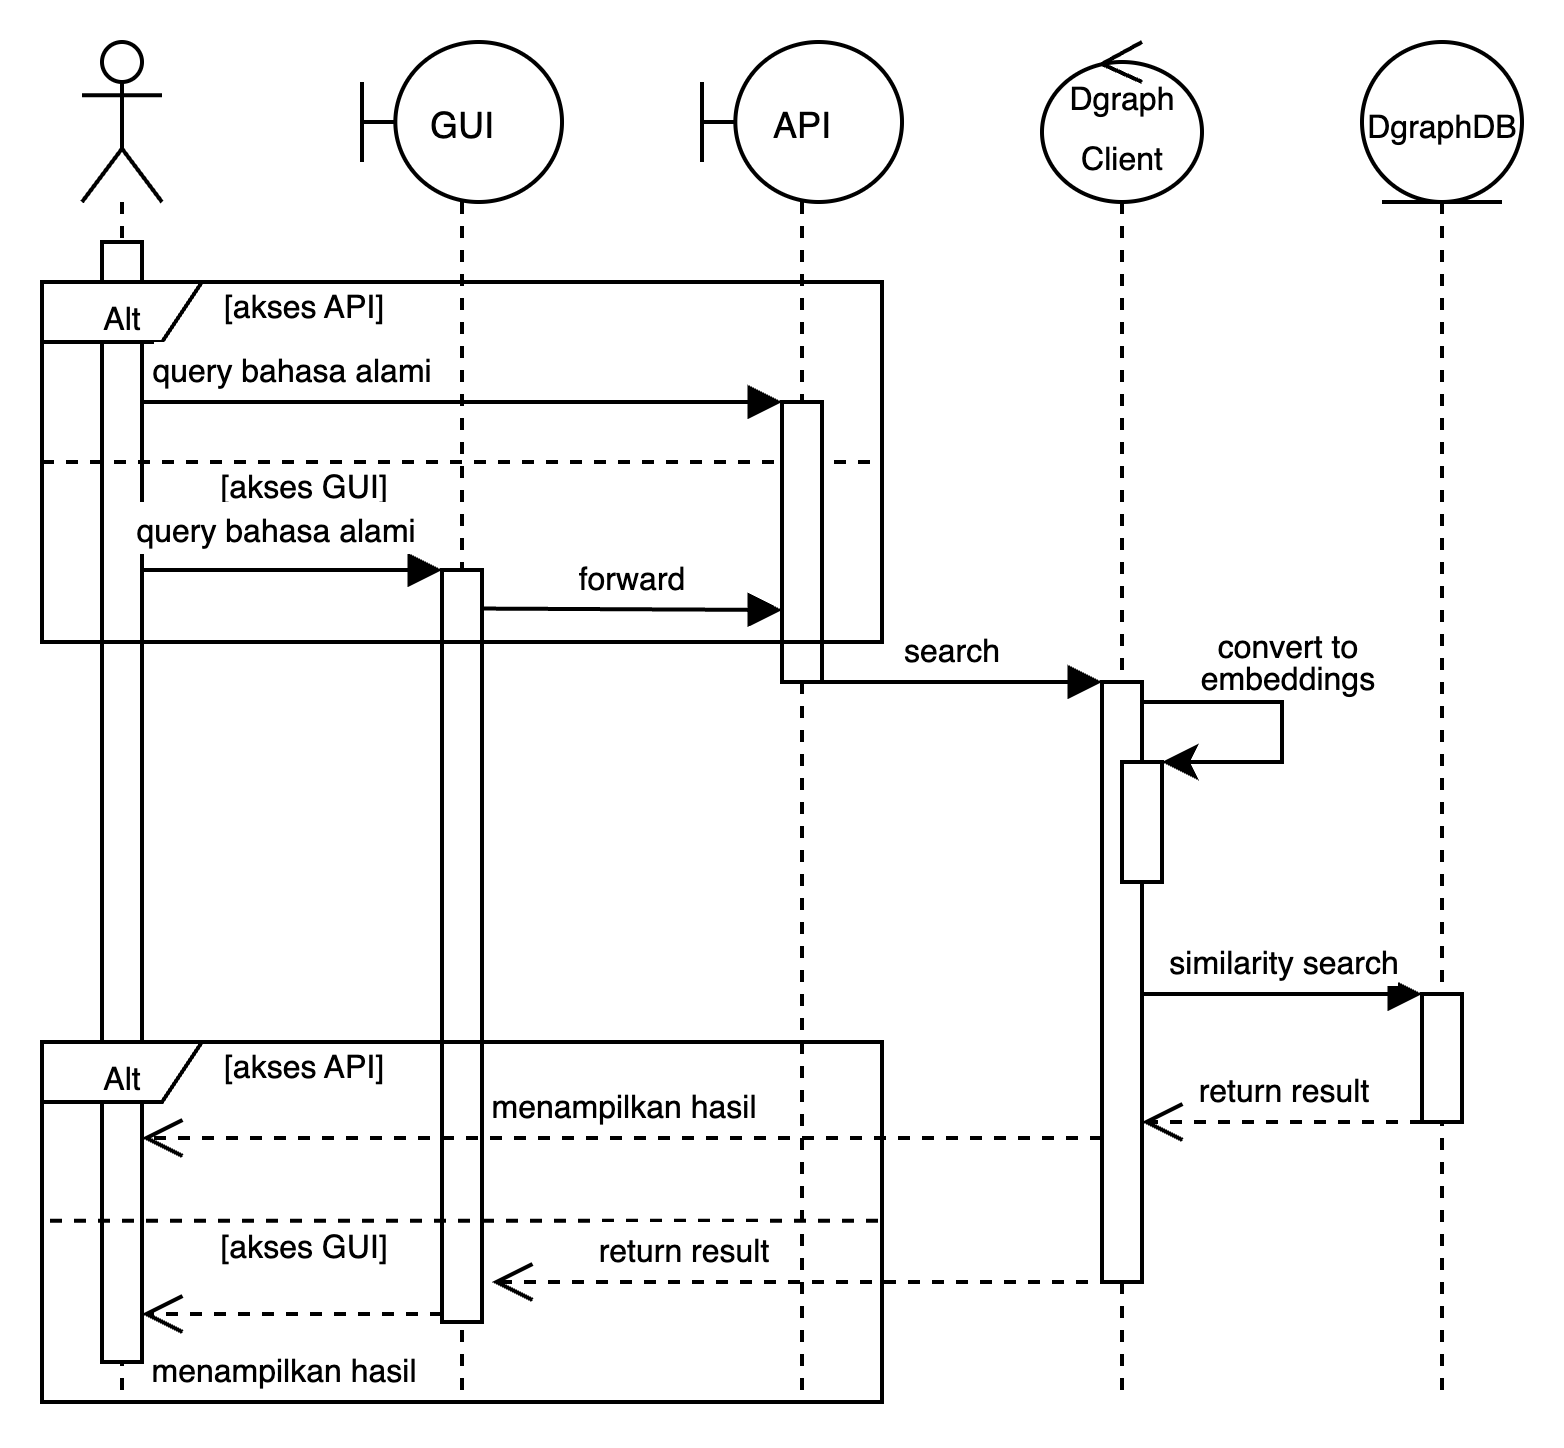
\includegraphics[width=0.7\textwidth]{resources/chapter-3/sequence-1.png}
    \caption{Alur Pencarian Smart Contract}
    \label{image:alur-pencarian-smart-contract}
\end{figure}


\subsubsection{Alur Mendapatkan Address Smart Contract}

Pengguna akan melakukan pencarian dengan menggunakan API atau GUI. Pengguna akan memasukkan dgraph ID yang didapatkan dari hasil pencarian Smart Contract. Data ID yang diterima akan diteruskan ke API lalu ke dgraph Client, yang akan melakukan query ke dalam Dgraph Database. Hasil pencarian yang didapatkan akan dikembalikan ke API dan ditampilkan kepada pengguna dalam bentuk tabel yang berisi informasi Smart Contract dengan dgraph ID yang dimasukkan oleh pengguna. Ilustrasi alur mendapatkan address Smart Contract dapat dilihat pada Gambar \ref{image:alur-mendapatkan-address-smart-contract}.

\begin{figure}[ht]
    \centering
    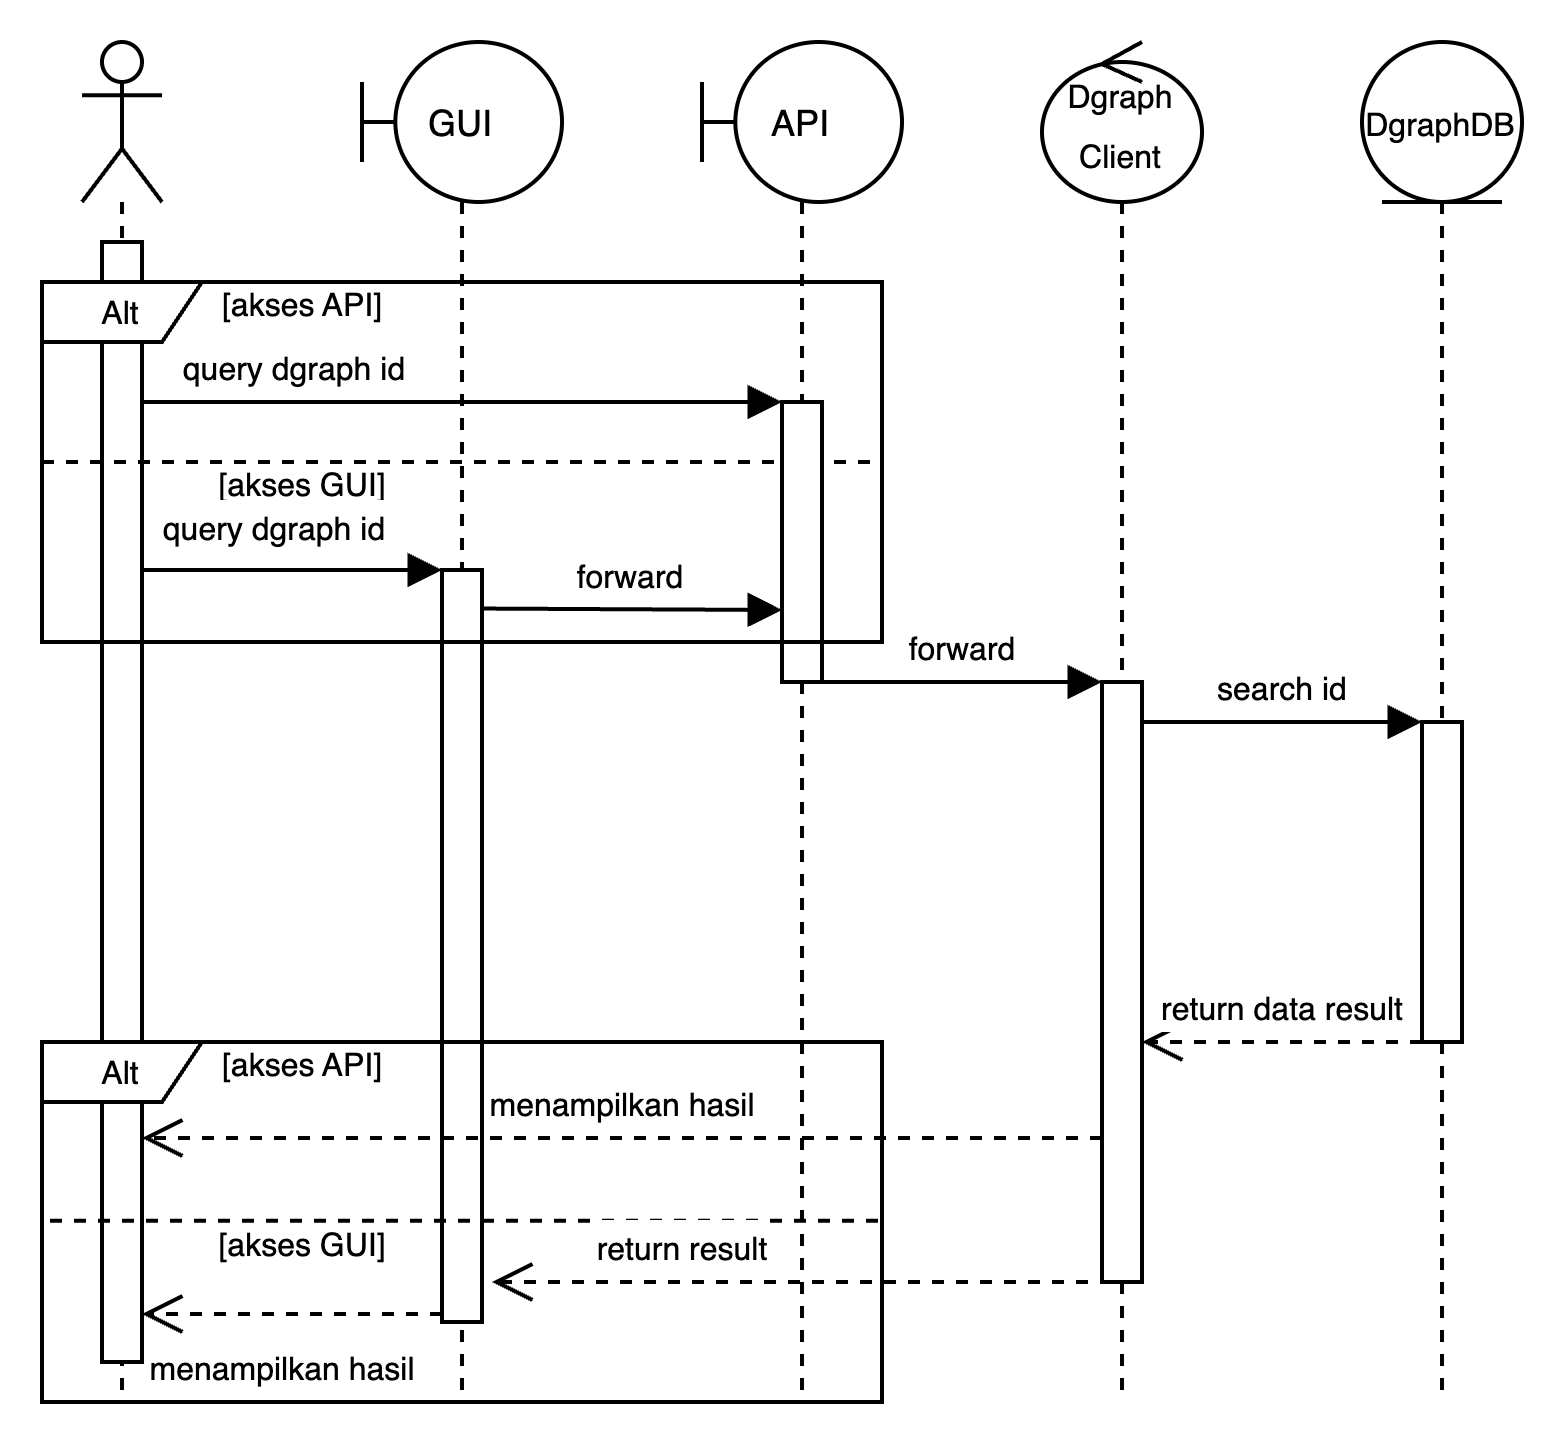
\includegraphics[width=0.7\textwidth]{resources/chapter-3/sequence-2.png}
    \caption{Alur Mendapatkan Address Smart Contract}
    \label{image:alur-mendapatkan-address-smart-contract}
\end{figure}

% \subsubsection{Alur Ekstraksi Data}

% \subsubsection{Alur Transformasi Data Menjadi Dgraph}

% \subsubsection{Alur Semantic Enrichment}

% \subsubsection{Alur Transformasi Data Menjadi Vector Embeddings}

% \subsubsection{Alur Penyimpanan Vector Embeddings}